\chapter{Introduction to Neural Networks}





\section{Artificial Neural Networks}
Nature has inspired many inventions, so it seems logical to look at the architecture of brain for inspiration on how to build an `intelligent machine'. This is the key idea which inspired Artificial Neural Networks (a.k.a. ANNs). In fact, an ANN is a computing system inspired by the biological neural networks which consitute animal brain. Therefore, an ANN is based on a set of connected units or nodes called artificial neurons for the comparison with biological neurons. Each connection, like the synapses in a biological brain, can transmit a signal from one artificial neuron to another. An artificial neuron that receives a signal can process it and then signal additional artificial neurons connected to it. For the sake of simplicity, from now on out we will denote ANN with Neural Networks, or more simply NNs.

In common NN implementations, neurons are arranged in consecutive layers, with the first and last ones called respectively input and output layers. Each layer can be fully connected with the subsequent layer, i.e. every single neuron of a layer is connected with all the neurons in the next layer. It is the case of a fully connected Neural Network. In other implementations, neurons can also be only partially connected in the meaning previously defined. For example, taking into account a network with 4 input neurons, 2 output neurons and a hidden layer with 8 neurons, the difference between the two types is highlighted by Figure \ref{fig:FCNN} and \ref{fig:NFCNN}.

\vspace{5mm}
\begin{minipage}[b]{0.45\linewidth}
    \centering
    % Fully Connected Neural Network
\begin{tikzpicture}[shorten >=1pt,->,draw=black!50, node distance=\layersep, scale=0.5]
    \tikzstyle{every pin edge}=[<-,shorten <=1pt]
    \tikzstyle{neuron}=[circle,fill=black!25,minimum size=10pt,inner sep=0pt]
    \tikzstyle{input neuron}=[neuron, fill=green!50];
    \tikzstyle{output neuron}=[neuron, fill=red!50];
    \tikzstyle{hidden neuron}=[neuron, fill=blue!50];
    \tikzstyle{annot} = [text width=4em, text centered]

    % Draw the input layer nodes
    \foreach \name / \y in {1,...,4}
    % This is the same as writing \foreach \name / \y in {1/1,2/2,3/3,4/4}
        \node[input neuron, draw=black!100, thick, pin=left:{\scriptsize In{[}\#\y{]}}] (I-\name) at (-\layersep,-1.5-1*\y) {};

    % Draw the hidden layer nodes
    \foreach \name / \y in {1,...,8}
        \path[yshift=0.5cm]
            node[hidden neuron,draw=black!100,thick] (H-\name) at (\layersep,-\y cm) {};

    % Draw the output layer node
    \node[output neuron,draw=black!100,thick,pin={[pin edge={->}]right:{\scriptsize Out{[}\#1{]}}}, right of=H-4] (O1) {};
    \node[output neuron,draw=black!100,thick,pin={[pin edge={->}]right:{\scriptsize Out{[}\#2{]}}}, right of=H-5] (O2) {};

    % Connect every node in the input layer with every node in the
    % hidden layer.
    \foreach \source in {1,...,4}
        \foreach \dest in {1,...,8}
            \path (I-\source) edge (H-\dest);

    % Connect every node in the hidden layer with the output layer
    \foreach \source in {1,...,8}
        \path (H-\source) edge (O1);
    \foreach \source in {1,...,8}
        \path (H-\source) edge (O2);

    % Annotate the layers
    \node[annot,above of=H-1, node distance=1.0cm] (hl) {Hidden layer};
    \node[annot,left of=hl] {Input layer};
    \node[annot,right of=hl] {Output layer};
\end{tikzpicture}
    \captionof{figure}{Fully connected ANN.}
    \label{fig:FCNN}
\end{minipage}
%
\hspace{2mm}
%
\begin{minipage}[b]{0.45\linewidth}
    \centering
    % Not Fully Connected Neural Network
\begin{tikzpicture}[shorten >=1pt,->,draw=black!50, node distance=\layersep, scale=0.5]
    \tikzstyle{every pin edge}=[<-,shorten <=1pt]
    \tikzstyle{neuron}=[circle,fill=black!25,minimum size=10pt,inner sep=0pt]
    \tikzstyle{input neuron}=[neuron, fill=green!50];
    \tikzstyle{output neuron}=[neuron, fill=red!50];
    \tikzstyle{hidden neuron}=[neuron, fill=blue!50];
    \tikzstyle{annot} = [text width=4em, text centered]

    % Draw the input layer nodes
    \foreach \name / \y in {1,...,4}
    % This is the same as writing \foreach \name / \y in {1/1,2/2,3/3,4/4}
        \node[input neuron, draw=black!100, thick, pin=left:{\scriptsize In{[}\#\y{]}}] (I-\name) at (-\layersep,-1.5-1*\y) {};

    % Draw the hidden layer nodes
    \foreach \name / \y in {1,...,8}
        \path[yshift=0.5cm]
            node[hidden neuron,draw=black!100,thick] (H-\name) at (\layersep,-\y cm) {};

    % Draw the output layer node
    \node[output neuron,draw=black!100,thick,pin={[pin edge={->}]right:{\scriptsize Out{[}\#1{]}}}, right of=H-4] (O1) {};
    \node[output neuron,draw=black!100,thick,pin={[pin edge={->}]right:{\scriptsize Out{[}\#2{]}}}, right of=H-5] (O2) {};

    % Connect every node in the input layer with every node in the
    % hidden layer.
    
    \foreach \dest in {1,2}
        \path (I-1) edge (H-\dest);
    \foreach \dest in {3,4}
        \path (I-2) edge (H-\dest);
    \foreach \dest in {5,6}
        \path (I-3) edge (H-\dest);
    \foreach \dest in {7,8}
        \path (I-4) edge (H-\dest);

    % Connect every node in the hidden layer with the output layer
    \foreach \source in {1,...,8}
        \path (H-\source) edge (O1);
    \foreach \source in {1,...,8}
        \path (H-\source) edge (O2);

    % Annotate the layers
    \node[annot,above of=H-1, node distance=1.0cm] (hl) {Hidden layer};
    \node[annot,left of=hl] {Input layer};
    \node[annot,right of=hl] {Output layer};
\end{tikzpicture}
    \captionof{figure}{Partially connected ANN.}
    \label{fig:NFCNN}
\end{minipage}
\vspace{5mm}

We will consider fully connected NNs to explain in a more technical manner their working principles. In particular, we will consider a network composed of a number of layers $L$. A Neural Network can be described mathematically by the composition of several function (nested units) associated to a certain layer:
%
\begin{equation}
    f_\mathrm{NN}(\vec{x}) = f \circ g \circ h \circ \dots \circ \vec{x} = f(g(h(\dots(\vec{x}))))
\end{equation}
%
with $\vec{x}$ the input of the NN and $f_\mathrm{NN}$ its output. The units in this representation can be of two kinds:
\begin{itemize}
    \item Linear transformations:
    %
    \begin{equation}
        h(\vec{x}) = \mathbf{w}^l\vec{x} + \vec{b}^l
    \end{equation}
    %
    where:
    \begin{itemize}
        \item[$\triangleright$] $\mathbf{w}^l$ is a matrix of free parameters, called weights, whose elements $[\mathbf{w}]_{i,j}^l$ are the connections values between the $j^\text{th}$ neuron in the $(l-1)^\text{th}$ layer and the $i^\text{th}$ neuron in the $l^\text{th}$ layer.
        \item[$\triangleright$] $\vec{b}^l$ is a vector of free parameters, called biases, of the neurons in the $l^\text{th}$ layer.
    \end{itemize}
    
    \item Non-linear transformations, which don't depend on free parameters:
    %
    \begin{equation}
        g(\vec{x}) = [g(x_1),\dots,g(x_\mathrm{N})]
    \end{equation}
\end{itemize}

It is possible to deduce through this formalism that a Neural Network is a way to parametrize a set of functions, whose elements are spanned by weights and biases. Given the number of layers $\mathrm{L}$ of the NN, this set will be denoted as $\mathcal{F}_\mathrm{L}$:
%
\begin{equation}
    \mathcal{F}_\mathrm{L} = \{ f_\mathrm{NN}(x;\mathbf{w},\vec{b}), \ \forall \ \mathbf{w},\vec{b} \}
\end{equation}
%
The question of interest now is how to find the parameters $\mathbf{w}$ and $\vec{b}$ that suit best to our purpose. It is possible to achieve this accomplishment through a process called training, which is one of the key ideas behind the philosophy of Neural Networks and Deep Learning. Hence we need to implement an algorithm capable of updating the free parameters of the net to male them suitable to describe a dataset $\mathcal{D}$ given to the input layer. Moreover, a good choice of the architecture of the NN, of the algorithm and of the weights and biases could generalize the results of the procedure to a bigger dataset $\Tilde{\mathcal{D}}$.

In the following sections a step by step procedure of the training process will be explained. Moreover, several tecniques will be listed, considering that there isn't a fixed scheme in the algorithm, but a certain choice can fit better to a certain problem than another one.



\begin{comment}
\section{Training a Neural Network}
In practice applications, given a set of data $\mathcal{D}$ whose tendency and distribution we want to describe, the philosophy behind Neural Networks and Deep Learning is finding the best choice of free parameters that describes $\mathcal{D}$. In order to accomplish this goal, we have to implement an algorithm which updates the free parameters, i.e. weights and biases, to make them suitable to describe the dataset and its generalization to a bigger one.
\end{comment}



\section{Choice of NN architecture and activation functions}
% Oreilly p. 272
The flexibility of NNs is also one of their main drawbacks. In fact, there are many hyperparameters to tweak. But what do we mean with the word hyperparameter? It was previously described that a NN can parametrize a wide set of functions with the right choice of weights and biases, which are the free parameters of the net. however, there are many other parameters we have to consider and tune if we want to answer our demands. They are going to be presented step by step in the implementation of the learning procedure.

The first thing we have to take into account in the development of a NN is its achitecture, i.e. the number of layers and the number of neurons for each layer. The architecture of a NN is the first of the hyperparameters of the net. After this step, the activation functions for every layer are to be selected among a wide variety of solutions.
%Depending on the complexity of the problem we have to solve, we can choose a NN composed of several hidden layers. In general, the more the dataset to generalize is big and complex, the greater the number of layers requires will be. In fact, a NN with more layers is capable to describe a wider set of functions $\mathcal{F}_\mathrm{L}$.

\subsection{Number of hidden layers}
% Oreilly p. 273
For many problems, it is possible to begin with a single hidden layer and get reasonable results. As a matter of facts, it can be proved that a NN just like the previous one can model even the most complex functions provided it has enough neurons. This was the reason for which many researchers thought for a long time that there was no need to investigate any deeper NNs. However deep networks (i.e. with more than one hidden layer) are much more powerful than shallow ones. They have a much higher parameter efficiency because they are capable of modelling complex functions using exponentially fewer neurons than shallow nets. Through this expedient the train process could be sped up for the fewer number of free parameters.

Another important reason to prefer deep networks for more complex problems has a heuristic justification. In fact, this kind of NNs is more adaptable to the hierarchical structure of real-world data. Lower hidden layers model low-level features, intermediate hidden layers combine these low-level features to model intermediate-level features, and the highest hidden layers and the output layer combine these intermediate features to model high-level features. Moreover, not only does this hierarchical architecture help deep NNs converge faster to a good solution, it also improves their ability to generalize to new datasets.

In summary, for many problems it is possible to start with just one or two hidden layers and it will work just fine. For more complex problems, the strategy is to gradually raise the number of hidden layers until the model starts overfitting the training dataset.



\subsection{Number of neurons per hidden layer}
% Oreilly p. 274
Obviously the number of neurons in the input and output layers is determined by the type of input and output required by the problem. For the hidden layers, a common practice is to size them to form a funnel, with fewer and fewer neurons at each layer. This possible architecture is motivated by the fact that many low-level features can combine into far fewer high-level features. However, this practice is not as common now and it is a valid solution to use the same size for all hidden layers. The advantage of the last practice is that there is only one hyperparameter to tune for the number of neurons per layer, instead of one hyperparameter per layer. Just like for the number of layers, we can try to increase the number of neurons gradually until the network starts overfitting the data.

In general, it is more productive to increase the number of layers than the number of neurons per layer. Finding the perfect amount of neurons is quite difficult. A simpler approach is to pick a model with more layers and neurons than we actually need and then stop the training process earlier in order to prevent it from overfitting. It is worth to employ also some regularization techniques that will be presented in the following sections.


% Another approach is to add more neurons in a single layer and reducing the number of hidden layers. There isn't a systematic approach, but in general the more the NN is complex, the greater the training time required to learn from the dataset will be. Moreover, a more complex NN needs a number of data quite large while sometimes we have at our disposal a limited number of samples.

% Choosing the architecture of the NN, the first thing to do is to select the number of neurons in the input and output layers. The number of neurons in the input layer is the number of input data given to the net in every step of the training routine. The number of neurons in the output layer depends on the results we want to reproduce. There could be just one neuron if the purpose is to have in output a single variable. There could be $n$ neurons if ours is a classification problem and the net must be capable of choosing among $n$ possibilities.

% After we have fixed the number of layers $L$ and the neurons for each layer, the next thing to do is selecting an activation function for every layer. There is a quite large variety of possibilities for this selection. In the following part some of the most common solutions will be presented along with their advantages and disadvantages.



\subsection{Activation functions}
% Oreilly p. 274
For each training instance, the algorithm employed feeds it to the network and computes the output of every neuron in each consecutive layer. This output is given by a function called 'activation'. The selection of the activation functions for every layer is not only pretty important if we want to get excellent results, but it is also crucial to speed up the computation, in particular if the expected training time is relative long. It is possible to assemble a network with a different activation per layer depending on what we want to do. Several functions that suits to the purpose are presented below along with their advantages and disadvantages.

\vspace{0.2cm}
\noindent
\begin{minipage}[t]{0.4\textwidth}
%\centering
\strut\vspace*{-\baselineskip}%\newline
\begin{comment}
\begin{gnuplot}[terminal=epslatex, terminaloptions=color dashed, terminaloptions={size 8cm,5cm}]
a(x) = x>0 ? 1 : -1
set samples 10000
set key at -1.4,1.25

set xrange[-5.0:5.0]
set yrange[-1.5:1.5]

set format x "\%1.1f"
set format y "\%1.1f"

plot a(x) lc rgb "red" lw 4
\end{gnuplot}
\end{comment}

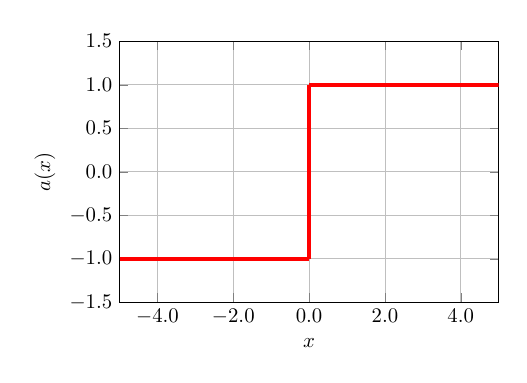
\begin{tikzpicture}[scale=0.75]
\begin{axis}[
width=8cm, height=6cm,
xmin=-5, xmax=5,
ymin=-1.5, ymax=1.5, 
grid, 
xlabel=$x$, ylabel=$a(x)$,
xtick = {-4.0,-2.0,0,2.0,4.0},
ytick = {-1.5,-1.0,-0.5,0,0.5,1.0,1.5},
y tick label style={/pgf/number format/.cd,%
        fixed,
        fixed zerofill,
        precision=1},
x tick label style={/pgf/number format/.cd,%
        fixed,
        fixed zerofill,
        precision=1}
]

\draw[line width=2.pt,color=red] (-5,-1) -- (0,-1);
\draw[line width=2.pt,color=red] (0,-1) -- (0,1);
\draw[line width=2.pt,color=red] (0,1) -- (5,1);

% \addplot[red,smooth] gnuplot[id=step]{x>0 ? 1 : -1};

% \addplot[red,smooth] {tanh(x)};

\end{axis}
\end{tikzpicture}
\label{fig:STEP}
\end{minipage}%
\begin{minipage}[t]{0.6\textwidth}
\textbf{Step function}
\begin{flalign}
    a(x) = \begin{cases} 1 & x\ge0 \\ -1 & x<0\end{cases} &&
\end{flalign}
A neuron with this activation is called linear threshold unit (LTU). A single LTU can be used for simple linear binary classification problems. In general a network of LTU could not be sufficient to get reasonable results.
\end{minipage}


\noindent
\begin{minipage}[t]{0.4\textwidth}
%\centering
\strut\vspace*{-\baselineskip}\newline
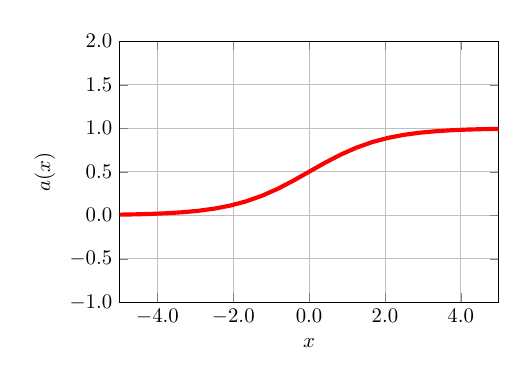
\begin{tikzpicture}[scale=0.75]
\begin{axis}[
width=8cm, height=6cm,
xmin=-5, xmax=5,
ymin=-1.0, ymax=2.0, 
grid, 
xlabel=$x$, ylabel=$a(x)$,
xtick = {-4.0,-2.0,0,2.0,4.0},
ytick = {-1.0,-0.5,...,2.0},
y tick label style={/pgf/number format/.cd,%
        fixed,
        fixed zerofill,
        precision=1},
x tick label style={/pgf/number format/.cd,%
        fixed,
        fixed zerofill,
        precision=1}
]

\addplot[line width=2.pt,color=red]{1/(1+e^(-x))};

% \addplot[red,smooth] gnuplot[id=step]{x>0 ? 1 : -1};

% \addplot[red,smooth] {tanh(x)};

\end{axis}
\end{tikzpicture}
\label{fig:SIGMOID}
\end{minipage}%
\begin{minipage}[t]{0.6\textwidth}
\textbf{Sigmoid function}
\begin{flalign}
    a(x) = \frac{1}{1+\operatorname{e}^{-x}} &&
\end{flalign}
The sigmoid function has a well-defined nonzero derivative everywhere, allowing the algorithms presented in next sections to work properly and make progresses at every step. It is probably one of the most employed for its properties.
\end{minipage}


\noindent
\begin{minipage}[t]{0.4\textwidth}
%\centering
\strut\vspace*{-\baselineskip}\newline
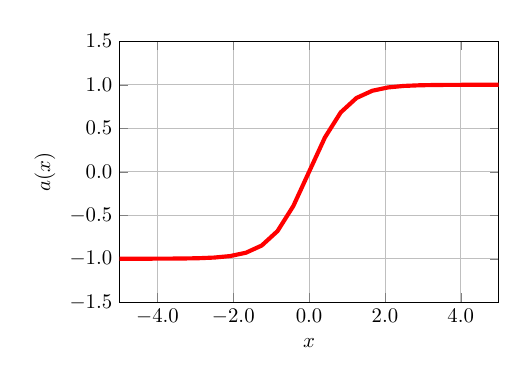
\begin{tikzpicture}[scale=0.75]
\begin{axis}[
width=8cm, height=6cm,
xmin=-5, xmax=5,
ymin=-1.5, ymax=1.5, 
grid, 
xlabel=$x$, ylabel=$a(x)$,
xtick = {-4.0,-2.0,0,2.0,4.0},
ytick = {-1.5,-1.0,...,1.5},
y tick label style={/pgf/number format/.cd,%
        fixed,
        fixed zerofill,
        precision=1},
x tick label style={/pgf/number format/.cd,%
        fixed,
        fixed zerofill,
        precision=1}
]

\addplot[line width=2.pt,color=red]{tanh(x)};

% \addplot[red,smooth] gnuplot[id=step]{x>0 ? 1 : -1};

% \addplot[red,smooth] {tanh(x)};

\end{axis}
\end{tikzpicture}
\label{fig:TANH}
\end{minipage}%
\begin{minipage}[t]{0.6\textwidth}
\textbf{Hyperbolic tangent function}
\begin{flalign}
    a(x) = \tanh{x} &&
\end{flalign}
Just like the sigmoid function it is S-shaped, continuous and differentiable, but the difference is that the output value ranges from -1 to 1 (instead of 0 to 1), which tends to make each layer's output more or less normalized at the beginning of training. This often help to speed up convergence.
\end{minipage}


\noindent
\begin{minipage}[t]{0.4\textwidth}
%\centering
\strut\vspace*{-\baselineskip}\newline
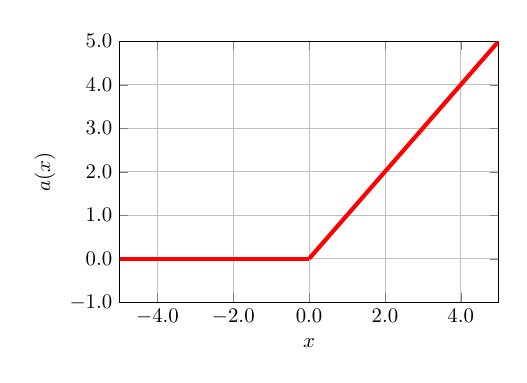
\begin{tikzpicture}[scale=0.75]
\begin{axis}[
width=8cm, height=6cm,
xmin=-5, xmax=5,
ymin=-1.0, ymax=5.0, 
grid, 
xlabel=$x$, ylabel=$a(x)$,
xtick = {-4.0,-2.0,0,2.0,4.0},
ytick = {-1.0,0.0,...,5.0},
y tick label style={/pgf/number format/.cd,%
        fixed,
        fixed zerofill,
        precision=1},
x tick label style={/pgf/number format/.cd,%
        fixed,
        fixed zerofill,
        precision=1}
]

\draw[line width=2.pt,color=red] (-5,0) -- (0,0);
\addplot[line width=2.pt,color=red,domain=0:5]{x};

% \addplot[red,smooth] gnuplot[id=step]{x>0 ? 1 : -1};

% \addplot[red,smooth] {tanh(x)};

\end{axis}
\end{tikzpicture}
\label{fig:RELU}
\end{minipage}%
\begin{minipage}[t]{0.6\textwidth}
\textbf{ReLU function}
\begin{flalign}
    a(x) = \operatorname{max}(0,x) &&
\end{flalign}
It is continuous but not differentiable at $x=0$. However, in practice it works very well and has the advantage of being very fast to compute. It does not have a maximum output value.
\end{minipage}


\begin{comment}
{%
\setlength\intextsep{0pt}
\begin{wrapfigure}{l}{0.4\textwidth}
    % \vspace{-12mm}
    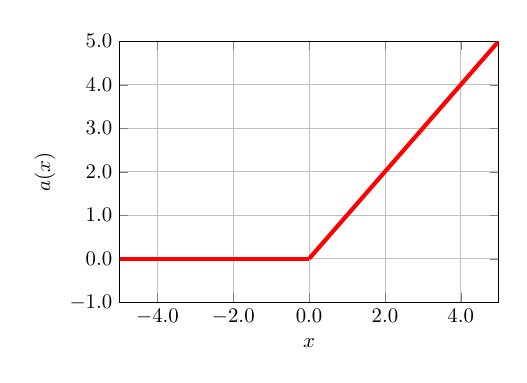
\begin{tikzpicture}[scale=0.75]
\begin{axis}[
width=8cm, height=6cm,
xmin=-5, xmax=5,
ymin=-1.0, ymax=5.0, 
grid, 
xlabel=$x$, ylabel=$a(x)$,
xtick = {-4.0,-2.0,0,2.0,4.0},
ytick = {-1.0,0.0,...,5.0},
y tick label style={/pgf/number format/.cd,%
        fixed,
        fixed zerofill,
        precision=1},
x tick label style={/pgf/number format/.cd,%
        fixed,
        fixed zerofill,
        precision=1}
]

\draw[line width=2.pt,color=red] (-5,0) -- (0,0);
\addplot[line width=2.pt,color=red,domain=0:5]{x};

% \addplot[red,smooth] gnuplot[id=step]{x>0 ? 1 : -1};

% \addplot[red,smooth] {tanh(x)};

\end{axis}
\end{tikzpicture}
    \label{fig:STEP}
\end{wrapfigure}
\noindent \\ \bf{ReLU function}
\begin{flalign}
    a(x) = \operatorname{max}(0,x) &&
\end{flalign}\\ \\ \\ \\ \\
}
\end{comment}





\section{Loss functions}
% Deep Learning Book p. 79
Another key concept of the training algorithm is evaluating if the network is working right. For this purpose, we have to quantify how much network predictions are wrong and we can do it by choosing a 'loss function', or also called 'cost function' or 'objective function'. There is a wide variety also for this kind of functions, but they are more related to the problem to solve than the activations. Choosing a wrong loss means getting worse results for our model. Sometimes a loss function is built from scratch to solve a single problem, so it is built ad hoc for a purpose.

In general, most deep learning algorithms involve optimization if some sort. Optimization referes to the task of either minimizing or maximizing a function $f(x)$ by altering $x$. A more common practice is to phrase the problem in terms of minimizing $f(x)$. Maximization is equivalent to minimization processes if we consider the function $-f(x)$.

A selection of possible techniques that can be used for optimization is presented in section 2.5. In the space below some of the most common loss functions are given along with the terms of use.


% https://towardsdatascience.com/common-loss-functions-in-machine-learning-46af0ffc4d23
\begin{itemize}
    \item[$\triangleright$] \textbf{Mean Squared Error (MSE or L2 Loss)}:\\
    As the name suggests, Mean Square Error is measured as the average of squared difference between predictions $y_i$ and actual observations $\hat{y_i}$.
    \begin{equation}
        L_{\mathrm{MSE}} = \frac{1}{n} \sum_{i=1}^{n} (y_i - \hat{y_i})^2
    \end{equation}
    It is only concerned with the average magnitude of error irrespective of their direction. However, due to squaring, predictions which are far away from actual values are penalized heavily in comparison to less deviated predictions. Plus MSE has nice mathematical properties which makes it easier to calculate gradients.
    
    \item[$\triangleright$] \textbf{Mean Absolute Error (MAE or L1 Loss)}:\\
    Mean absolute error is measured as the average of sum of absolute differences between predictions $y_i$ and actual observations $\hat{y_i}$.
    \begin{equation}
        L_{\mathrm{MAE}} = \frac{1}{n} \sum_{i=1}^{n} \abs{y_i - \hat{y_i}}^2
    \end{equation}
    Like MSE, this as well measures the magnitude of error without considering their direction. Unlike MSE, MAE needs more complicated tools such as linear programming to compute the gradients. Plus MAE is more robust to outliers since it does not make use of square.
    
    % https://ml-cheatsheet.readthedocs.io/en/latest/loss_functions.html
    % Deep Learning Book p. 73, 129
    \item[$\triangleright$] \textbf{Cross Entropy Loss (Negative Log Likelihood)}:\\
    This is the most common setting for classification problems. Cross-entropy loss increases as the predicted probability for a class out of $M$ possibilities diverges from the actual label.
    \begin{equation}
        H(y_o,p_o) = - \sum_{i=1}^{M} y_{o,i} \log{p_{o,i}}
    \end{equation}
    Terminology:\\
    $M = \text{Number of classes}$\\
    $y = \text{Binary indicator (0 or 1) if class label $i$ is the correct classification for observation $o$}$\\
    $p = \text{predicted probability observation $o$ is of class $i$}$\\
    So, when the label $y_{o,i}$ is equal to 1, the other terms of the sum disappear. An important aspect of this is that Cross Entropy Loss penalizes heavily the predictions that are confident but wrong.
    
    % Deep Learning Book p. 72
    % http://www.awebb.info/blog/cross_entropy
    \item[$\triangleright$] \textbf{Kullback-Leibler Divergence (KL)}:\\
    In mathematical statistics, the Kullback–Leibler Divergence (also called relative entropy) is a measure of how one probability distribution is different from a second, reference probability distribution. translated in terms of our optimization problem:
    \begin{equation}
        D_{\mathrm{KL}}(p||q) = - \left( \sum_{i=1}^{M} y_{o,i} \log{p_{o,i}} - \sum_{i=1}^{M} y_{o,i} \log{y_{o,i}} \right)
    \end{equation}
\end{itemize}





% http://neuralnetworksanddeeplearning.com/chap2.html
\section{Backpropagation algorithm}
% Deep Learning Book p. 197
% Deep Learning Book p. 204-205
When we use a feedforward neural network to accept an input $x$ and produce an output $\hat{y}$, information flows forward through the network. The input $x$ provides the initial information that then propagates up to the hidden units at each layer and finally produces $\hat{y}$. This is called forward propagation. 

During training, forward propagation can continue onward until it produces a scalar loss $L(\mathbf{w},\vec{b}$. The backpropagation algorithm, often simply called backprop, allows the information from the loss to then flow backward through the network in order to compute the gradient of the loss respect to the free parameters $\mathbf{w}$ and $\vec{b}$. Numerically evaluating such an expression can be computationally expensive. The backpropagation algorithm does so using a simple and inexpensive procedure.

The fundamental equations of the algorithm are presented below.
\begin{align}
    \delta^L &= \nabla_a C \odot \sigma^{\prime}(z^L)   \\
    \delta^l &= [(\mathbf{w}^{l+1})^T \delta^{l+1}] \odot \sigma^{\prime}(z^L)    \\
    \frac{\partial C}{\partial b^{l}_{i}} &= \delta^{l}_{i}  \\
    \frac{\partial C}{\partial \mathbf{w}^{l}_{ik}} &= a^{l-1}_{k} \delta^{l}_{i}
\end{align}

Translated in form of pseudo-code, the backpropagation algorithm appears like the one in the space below. It has to be specified that this algorithm is adapted for a fully connected network. In the case of a not-fully connected network the code becomes a bit more complex, but the concept behind is the same.

% Deep Learning Book p.205 (copiato e rimodellato)
\begin{algorithm}[H]
\caption{Forward propagation through a typical deep neural network and the computation of the cost function. The loss $L(\hat{y},y)$ depends on the output $\hat{y}$ and on the target $y$. The symbol $\theta$ will be used to indicate both weights and biases.}\label{FORWARD_PROPAGATION}
\begin{algorithmic}[1]
\Require Network depth, $l$
\Require $\mathbf{w}^{(i)}$, $i \in \{1,\dots,l\}$, the weight matrices of the model
\Require $b^{(i)}$, $i \in \{1,\dots,l\}$, the bias parameters of the model
\Require $x$, the input to the process
\Require $y$, the target output

\Procedure{Forward propagation}{$x$}%\Comment{The g.c.d. of a and b}

\State $h^{(0)} = x$

\For{$k=1,\dots,l$}
\State $a^{(k)} = b^{(k)} + \mathbf{w}^{(k)} h^{(k)}$
\State $h^{(k)} = f(a^{(k)})$
\EndFor

\State $\hat{y} = h^{(l)}$

\State \textbf{return} $\hat{y}$, $L(\hat{y},y)$
\EndProcedure
\end{algorithmic}
\end{algorithm}


% Deep Learning Book p.206 (copiato e rimodellato)
\begin{algorithm}[H]
\caption{Backward computation for the deep neural network of Algorithm \ref{FORWARD_PROPAGATION}, which uses, in addition to the input $x$, a target $y$. This computation yields the gradients on the activations $a^{(k)}$ for each layer $k$, starting from the output layer and going backwards to the first hidden layer. From these gradients, which can be interpreted as an indication of how each layer's output should change to reduce error, one can obtain the gradient on the parameters of each layer.}\label{BACKWARD_COMPUTATION}
\begin{algorithmic}[1]
\Procedure{Backward computation}{$x$} \Comment After the forward computation

\State $g \gets \nabla_{\hat{y}}L = \nabla_{\hat{y}}L(\hat{y},y)$\Comment Compute the gradient on the output layer

\For{$k=l,l-1,\dots,1$}
\State $g \gets \nabla_{a^{(k)}}L = g \odot f^{\prime}(a^{(k)})$
\State $\nabla_{b^{(k)}}L = g$
\State $\nabla_{\mathbf{w}^{(k)}}L = g h^{(k-1)~T}$
\State $g \gets \nabla_{h^{(k-1)}}L = \mathbf{w}^{(k)~T} g$
\EndFor

\State \textbf{return} $\nabla_{b^{(k)}}L$, $\nabla_{\mathbf{w}^{(k)}}L$, $k \in \{1,\dots,l\}$
\EndProcedure
\end{algorithmic}
\end{algorithm}





\section{Updating free parameters: Optimizers}
Now that we have a solid method to compute the derivatives respect to free parameters of the loss function $L$, we can update weights and biases according to the derivatives. In fact, those quantities can be seen as a measure of how much the parameters are to be changed in order to get results that resemble the output. The basic idea is to change $\mathbf{w}$ and $\vec{b}$ of a quantity equals to the corrisponding derivative multiplied by $-\eta$, where $\eta$ is another hyperparameter called learning rate. It is in general a small number that represents the speed of the learning process. It is fixed at the beginning of the procedure for some algorithms, for others it is variable during the training process, starting from a predefined value.

% OReilly p. 297
We focus now on the algorithms that execute the updaing phase of the parameters. They are called optimizers, just like the title of the section suggests and also for them there is a wide variety of choices. Some of them are still under study because their generalization power has not be proven completely. This is the case of "adam" algorithm. We'll start to explain one the simplest, the Stochastic Gradient Descent (SGD), and then we'll introduce the so called fast optimizers. training a very large deep neural network can be painfully slow, but this kind of optimizers, along with some other techniques, gives a huge boost to the computation.

\subsection{An example of algorithm with fixed learning rate}
% Deep Learning Book p.286 (copiato e rimodellato)
\begin{algorithm}[H]
\caption{Stochastic Gradient Descent (SGD) update at training iteration $k$}\label{SGD}
\begin{algorithmic}[1]
\Require Learning rate $\eta_{k}$
\Require Initial parameter $\theta$

\Procedure{SGD}{$\{x^{(i)}\}_{i=1,\dots,n}$} \Comment Take as input a dataset of $n$ elements

\While{stopping criterion not met}
\State Sample a minibatch $\{x^{(1)},\dots,x^{(m)}\}$ from the training set with corresponding targets $y^{(i)}$.
\State $\hat{g} \gets + \frac{1}{m} \nabla_{\mathbf{\theta}} \sum_{i} L(f(x^{(i)};\mathbf{\theta}), y^{(i)})$ \Comment{Compute gradient estimate}
\State $\mathbf{\theta} \gets \mathbf{\theta} - \eta \hat{g}$
\EndWhile

\State \textbf{return} $\mathbf{\theta}$
\EndProcedure
\end{algorithmic}
\end{algorithm}



\subsection{An example of algorithm with adaptive learning rates}
\begin{comment}
                    % Deep Learning Book p.300 (copiato e rimodellato)
                    \begin{algorithm}[H]
                    \caption{RMSProp algorithm}\label{RMSPROP}
                    \begin{algorithmic}[1]
                    \Require Global learning rate $\eta$, decay rate $\rho$
                    \Require Initial parameter $\theta$
                    \Require Small constant $\delta$, usually $10^{-6}$, used to stabilize division by small numbers
                    \Require Minibatch dimension $m$
                    
                    \Procedure{RMSProp}{$\{x^{(i)}\}_{i=1,\dots,n}$} \Comment Take as input a dataset of $n$ elements
                    
                    \State Initialize accumulation variables $r=0$
                    
                    \While{stopping criterion not met}
                    \State Sample a minibatch $\{x^{(1)},\dots,x^{(m)}\}$ from the training set with corresponding targets $y^{(i)}$.
                    \State $\hat{g} \gets + \frac{1}{m} \nabla_{\mathbf{\theta}} \sum_{i} L(f(x^{(i)};\mathbf{\theta}), y^{(i)})$ \Comment{Compute gradient estimate}
                    \State $r \gets \rho r + (1-\rho)g \odot g$ \Comment Accumulate squared gradient
                    \State $\Delta \theta = - \frac{\epsilon}{\sqrt{\delta + r}} \odot g$ \Comment Compute parameter update
                    \State $\mathbf{\theta} \gets \mathbf{\theta} + \Delta \mathbf{\theta}$
                    \EndWhile
                    
                    \State \textbf{return} $\mathbf{\theta}$
                    \EndProcedure
                    \end{algorithmic}
                    \end{algorithm}
\end{comment}


% Deep Learning Book p.301 (copiato e rimodellato)
\begin{algorithm}[H]
\caption{Adam algorithm}\label{ADAM}
\begin{algorithmic}[1]
\Require Step size $\epsilon$ (suggested default: $0.001$)
\Require Exponential decay rates for moment estimates, $\rho_1$,$\rho_2$ $\in [0,1)$ (suggested defaults: $0.9$ and $0.999$ respectively)
\Require Small constant $\delta$, usually $10^{-8}$, used to stabilize division by small numbers
\Require Initial parameter $\theta$
\Require Minibatch dimension $m$

\Procedure{Adam}{$\{x^{(i)}\}_{i=1,\dots,n}$} \Comment Take as input a dataset of $n$ elements

\State Initialize $1^\text{st}$ and $2^\text{nd}$ moment variables, $s=0$, $r=0$
\State Initialize time step $t=0$

\While{stopping criterion not met}
\State Sample a minibatch $\{x^{(1)},\dots,x^{(m)}\}$ from the training set with corresponding targets $y^{(i)}$.
\State $\hat{g} \gets + \frac{1}{m} \nabla_{\mathbf{\theta}} \sum_{i} L(f(x^{(i)};\mathbf{\theta}), y^{(i)})$ \Comment{Compute gradient estimate}
\State $t \gets t+1$
\State $s \gets \rho_1 s + (1-\rho_1) g$    \Comment Update biased $1^\text{st}$ moment estimate
\State $s \gets \rho_2 r + (1-\rho_2) g \odot g$    \Comment Update biased $2^\text{nd}$ moment estimate
\State $\hat{s} \gets \frac{s}{1 - \rho^t_1}$   \Comment Correct bias in $1^\text{st}$ moment
\State $\hat{r} \gets \frac{r}{1 - \rho^t_2}$   \Comment Correct bias in $2^\text{nd}$ moment
\State $\Delta \theta = - \epsilon \frac{\hat{s}}{\sqrt{\hat{r}} + \delta}$ \Comment Compute parameter update
\State $\mathbf{\theta} \gets \mathbf{\theta} + \Delta \mathbf{\theta}$
\EndWhile

\State \textbf{return} $\mathbf{\theta}$
\EndProcedure
\end{algorithmic}
\end{algorithm}





\section{Advanced tecniques}
It is possible to improve performances of a Neural Network through some other techniques. In particular, those techniques become necessary when the model we want the net to learn is pretty much complex and so the architecture of the net too.



\subsection{Regularizers}
% Deep Learning Book p.106-107
Regularization is one of the central concerns of the field of machine learning, rivaled in its importance only by optimization. Regularization is any modification we make to a learning algorithm that is intended to reduce its generalization error but not its training error. In practice, the most common way to regularize a model that learns a function $f(x;\theta)$ is adding a penalty called regularizer to the cost function. An example employed when weight decay is applied to the parametes is the following one:
\begin{equation}
    \Omega(\mathbf{w}) = \mathbf{w}^\mathrm{T} \mathbf{w}
\end{equation}



\subsection{Dropout}
% OReilly p.309
The most popular regularizatioon technique for deep neural networks is arguably dropout. It was proposed by [ADD REFERENCE] in 2012 and further detailed in [ADD OTHER REFERENCE]; it has proven tobe successful.

It is a very simple algorithm: at every training step, every neuron (including the input neurons but excluding the output neurons) has a probability $p$ of being temporarily "dropped out", meaning it will be entirely ingnored during this training step, but it may be active during the next step. The hyperparameter $p$ is called the dropout rate and it is typically set to 50\%. After training, neurons don't get dropped anymore.

A possible explanation of the effectiveness of dropout could be given. Neurons trained with dropout can't co-adapt with their neughbouring neuron. They have to be useful as possible on their own. They can't rely excessively on just a few input neurons and so they must pay attention to each of their input neurons. They end up being less sensitive to slight changes in the inputs. In the end, we get a more robust network that generalizes better.



\subsection{Parameter initialization strategies}
If we want to get better results from training procedure and to decrease training time, it is crucial to adopt a good initialization strategy of the free parameters. If we start with a set of parameters quite near to the set that minimizes the loss function, the training algorithm will rapidly find the path towards the local/global minimum of the loss function.

Several initialization strategies have been developed in the research field of Deep Learning. In the space below some of them are presented:

\begin{itemize}
    \item \textbf{Xavier and He initialization}. \\
    The connection weights must be initialized randomly ad described in Table \ref{tab:XAVIER_HE_INITIALIZATIONS}, where $n=n_\text{inputs}$ and $m=n_\text{outputs}$ are respectively the number of input and output connections for the layer whose weights are being initialized (also called fan-in and fan-out). The distribution used to initialization has to be chosen between a normal distribution with mean 0 and standard deviation $\sigma$ and a uniform distribution between $-r$ and $r$. He initialization is the name given to this kind of initialization with ReLU activations.
    
    \begin{table}[h]
        \centering
        \begin{tabular}{c c c}
            \toprule
             Activation function    &   Uniform distribution $[-r,r]$   &   Normal distribution $(0,\sigma)$   \\
             \toprule
             Logistic   &
             $ \displaystyle
                 r = \sqrt{\frac{6}{n+m}}
             $    &
             $ \displaystyle
                 \sigma = \sqrt{\frac{2}{n+m}}
             $ \\
             Hyperbolic tangent   &
             $ \displaystyle
                 r = 4 \sqrt{\frac{6}{n+m}}
             $    &
             $ \displaystyle
                 \sigma = 4 \sqrt{\frac{2}{n+m}}
             $ \\
             ReLU   &
             $ \displaystyle
                 r = \sqrt{2} \sqrt{\frac{6}{n+m}}
             $    &
             $ \displaystyle
                 \sigma = \sqrt{2} \sqrt{\frac{2}{n+m}}
             $ \\
             \bottomrule
        \end{tabular}
        \caption{Xavier and He initializations.}
        \label{tab:XAVIER_HE_INITIALIZATIONS}
    \end{table}
\end{itemize}